\chapter{Concept Assessment}\label{cha:assessment}

    The assessment of this project is calculated based on the number of interaction and complexity levels achieved as described in Tables~\ref{tab:uilevels} and~\ref{tab:techlevels}. Illustrated in Table~\ref{tab:levelCompare} is the relation between the level of user interaction and the technical complexity. The blue dots indicate the complexity level required to achieve a specific level of interaction. For example, interaction level $\mathcal{I}4$ (intermediate) requires a complexity of $\mathcal{C}5$ in order to be implemented. The highlighted section denotes the completed objectives for this project.

    \newcommand{\bmark}{\hskip 0.5em $\color{igmrBlue}\bullet$ \hskip 0.5em}
    \newcommand{\nomark}{\hskip 0.5em $\color{shade30}\circ$ \hskip 0.5em}
    \newcommand{\cshade}{\cellcolor{shade10}}

    \begin{table}[htbp]
        \color{textColor}
        \centering	
        \begin{tabular}{ cr|cccccccccc }
             &&&&&&&&&& \\
            \multirow{8}{*}{\rotatebox[origin=c]{90}{Interaction $[\,\mathcal{I}\,]\ \longrightarrow$\ }} 

             & $\mathcal{I}6$ & \bmark & \bmark & \bmark & \bmark & \bmark & \bmark & \bmark & \bmark & \bmark & \\[1em]

             & $\mathcal{I}5$ & \bmark & \bmark & \bmark & \bmark & \bmark & \bmark & \bmark & \nomark & \nomark & \\[1em]

             & $\mathcal{I}4$ & \cshade \bmark & \cshade \bmark & \cshade \bmark & \cshade \bmark & \cshade \bmark & \nomark & \nomark & \nomark & \nomark & \\[1em]

             & $\mathcal{I}3$ & \cshade \bmark & \cshade \bmark & \cshade \bmark & \cshade \nomark & \cshade \nomark & \nomark & \nomark & \nomark & \nomark & \\[1em]

             & $\mathcal{I}2$ & \cshade \bmark & \cshade \bmark & \cshade \nomark & \cshade \nomark & \cshade \nomark & \nomark & \nomark & \nomark & \nomark & \\[1em]

             & $\mathcal{I}1$ & \cshade \bmark & \cshade \bmark & \cshade \nomark & \cshade \nomark & \cshade \nomark & \nomark & \nomark & \nomark & \nomark & \\[1em]
             
            \cline{2-11} 
             &&&&&&&&&& \\[-5pt]
             &  & $\mathcal{C}1$ & $\mathcal{C}2$ & $\mathcal{C}3$ & $\mathcal{C}4$ & $\mathcal{C}5$ & $\mathcal{C}6$ & $\mathcal{C}7$ & $\mathcal{C}8$ & $\mathcal{C}9$ & \\[0.5em]
             &  \multicolumn{10}{c}{Complexity $[\,\mathcal{C}\,]\ \longrightarrow$} \\
        \end{tabular}
        \caption{Relation between user interaction and increasing technical complexity.}
        \label{tab:levelCompare}
    \end{table}

    It is assumed that users  will vary depending on the application. A beginner user, $\mathcal{U}1$, will benefit from an intermediate interface, $\mathcal{I}4$, when learning \ac{ROS} concepts. However, a student with programming experience, $\mathcal{U}2$, will demand a more interactive \ac{ROS} playground, $\mathcal{I}5$ and above. Similarly, experienced users, $\mathcal{U}3$ and $\mathcal{U}4$ will require all \ac{ROS} tools to be available, $\mathcal{I}6$, to justify a migration to a web browser platform.

\section{Layer Progression}

    The following sections describe the chronological progression of layers to achieve the results highlighted with gray in Table~\ref{tab:levelCompare}. As observed in the table, the progression through the levels is not a linear path, but a series of steps in multiple directions.

    \vspace{1em}
    \begin{tcolorbox}[title=Note]
        \begin{minipage}[t]{0.87\linewidth}
            \vspace*{0pt}
            If the reader would like to follow along with the demonstrations
            provided in the following pages, it is recommended to visit 
            \href{https://ros2wasm.dev/}{\textsf{ros2wasm.dev}}.
            Throughout the text, links will be provided to redirect the reader 
            to specific examples.
        \end{minipage}\hfill%
        \begin{minipage}[t]{0.1\linewidth}
            \vspace*{0pt}
            
\includegraphics[height=\linewidth,width=\linewidth]{qr_ros2wasm.png}
        \end{minipage}
    \end{tcolorbox}


        \subsection{Complexity Level 1}

        The groundwork for achieving any sort of user interface with \ac{ROS} running on the browser, lies on the development of a compatible middleware implementation ($\mathcal{C}1$). The design of this middleware implementation has been described in Chapter~\ref{cha:rmw}. The three packages (\textsf{rmw-wasm-cpp}, \textsf{wasm-cpp}, and \textsf{wasm-js}) on their own, do not aid the user in interacting with \ac{ROS}.

        \vspace{0.5em}
        \begin{tcolorbox}[title=Example 1]
            \begin{minipage}[t]{0.87\linewidth}
                \vspace*{0pt}
                The source code for the custom middleware implementation packages can be found in the following repository:

                \href{https://github.com/ihuicatl/rmw_wasm/}{\textsf{https://github.com/ihuicatl/rmw\smallunderscore wasm/}}
            \end{minipage}\hfill%
            \begin{minipage}[t]{0.1\linewidth}
                \vspace*{0pt}
                
\includegraphics[height=\linewidth,width=\linewidth]{qr_rmw_wasm.png}
            \end{minipage}
        \end{tcolorbox}

        \subsection{Complexity Level 2}

        The next step in complexity, $\mathcal{C}2$, involves creating a \ac{ROS} package for testing and cross-compiling such package along with its dependencies. For simplicity, the test package follows the official \ac{ROS} tutorials for how to create a publisher and a subscriber that communicate with each other in C++~\cite{humbletutorial}. By having this standard baseline, this ensures that the behavior of the middleware implementation packages can be adjusted until it matches the expected behavior for a typical \ac{ROS} publisher and subscriber. The CMake instructions were modified for each executable in order to have a successful cross-compilation with Emscripten. 

        \vspace{0.5em}
        \begin{tcolorbox}[title=Example 2]
            \begin{minipage}[t]{0.87\linewidth}
                \vspace*{0pt}
                The testing package, \textsf{test-wasm}, used for this project can be found in the following repository:

                \href{https://github.com/ihuicatl/rmw_wasm/tree/main/test_wasm}{\textsf{https://github.com/ihuicatl/rmw\smallunderscore wasm/tree/main/test\smallunderscore wasm}}
            \end{minipage}\hfill%
            \begin{minipage}[t]{0.1\linewidth}
                \vspace*{0pt}
                
\includegraphics[height=\linewidth,width=\linewidth]{qr_test_wasm.png}
            \end{minipage}
        \end{tcolorbox}

        To replicate the process locally, a build script (\textsf{blasm}) is provided in Appendix~\ref{sec:apxblasm}. As prerequisites, it is necessary to have an active installation of Emscripten and a copy of the \ac{ROS} 2 source code in a workspace. Figure~\ref{fig:vcs} shows the recommended procedure for cloning all \ac{ROS} 2 packages by using a \ac{VCS} tool~\cite{rosinstall}.

        \begin{figure}[htbp]
            \centering
            \begin{lstlisting}[language=Bash]
cd ~/workspace/src
vcs import --input https://raw.githubusercontent.com/ros2/ros2/humble/ros2.repos .
\end{lstlisting}
            \caption{Cloning all \ac{ROS} 2 packages with \textsf{vcstool}.}
            \label{fig:vcs}
        \end{figure}

        An even simpler solution for new users to build packages is to use a GitHub workflow. An example of such workflow is given in Appendix~\ref{sec:apxworkflow}. By adding this script to a repository which includes the desired \ac{ROS} package to be built, the user can manually trigger this workflow to build the target package without the need to have a local build set up. Figure~\ref{fig:workflow} displays the interface for running the \textsf{build-package} workflow from GitHub.

        \begin{figure}[htbp]
            \centering
            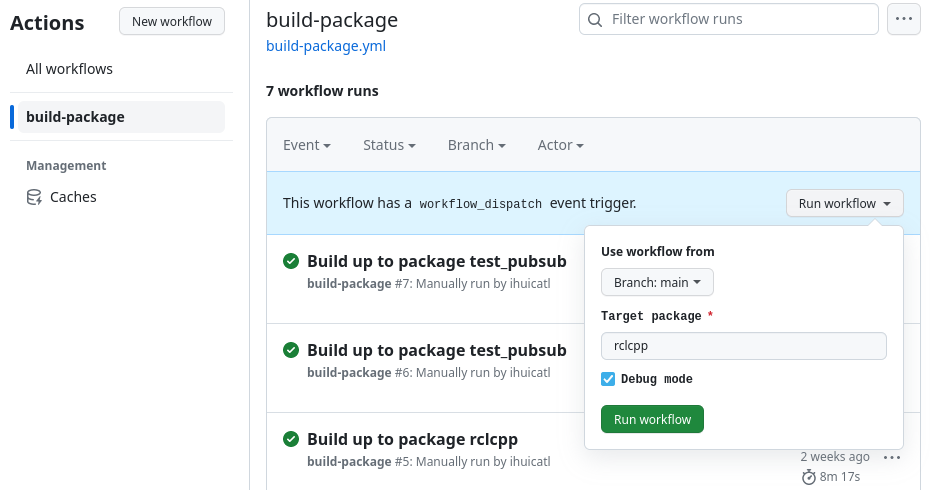
\includegraphics[width=\textwidth]{07_workflow.png}
            \caption{Triggering \textsf{build-package} workflow to build \textsf{rclcpp}.}
            \label{fig:workflow}
        \end{figure}

        \pagebreak

        The workflow runs through the following steps:

        \begin{enumerate}
            \item Install and activate \ac{emsdk}.
            \item Create a \ac{ROS} workspace.
            \item Install \textsf{vcstool}.
            \item Clone all \ac{ROS} 2 packages to the workspace.
            \item Removes unsupported packages such as the default middleware implementations, e.g. \textsf{FastRTPS}.
            \item Applies a patch to \textsf{rcutils} package.
            \item Creates a \textsf{conda} environment with the \textsf{colcon} packages installed.
            \item Runs the \textsf{blasm} script to build up to the target package.
            \item And uploads the artifacts.
        \end{enumerate}

        It is important to note that the artifacts are available for the user to download once the workflow has completed successfully. The contents of these artifacts will include any \ac{WASM}, JavaScript, and \ac{HTML} files generated by the target package during the build. However, the target package must contain executables in order for these files to be generated in the first place.

        This \textsf{build-package} workflow provides an overview of the procedure required to build packages locally or on an external server. Although the initial setup may seem laborious, automation tools can greatly simplify the process. 

        \vspace{0.5em}
        \begin{tcolorbox}[title=Example 3]
            \begin{minipage}[t]{0.87\linewidth}
                \vspace*{0pt}
                The source code for the described workflow can be found in the following repository:

                \href{https://github.com/ihuicatl/ros2wasm/blob/main/.github/workflows/build-package.yml}{\footnotesize{\textsf{https://github.com/ihuicatl/ros2wasm/blob/main/.github/workflows/build-package.yml}}}

                The reader is encouraged to fork the repository to test the workflow.
            \end{minipage}\hfill%
            \begin{minipage}[t]{0.1\linewidth}
                \vspace*{0pt}
                
\includegraphics[height=\linewidth,width=\linewidth]{qr_workflow.png}
            \end{minipage}
        \end{tcolorbox}

        \subsection{User Interaction Level 1: Non-Interactive}

        Once $\mathcal{C}1$ and $\mathcal{C}2$ levels are completed, this opens the door for minimal user interaction. With the testing package described above containing a publisher derived from the \ac{ROS} tutorials, a \ac{WASM} and a JavaScript are generated when cross-compiling the publisher executable. By creating a bare bones \ac{HTML} page, the publisher (\textit{talker}) can be run on the browser.

        \begin{figure}[htbp]
            \begin{lstlisting}[language=html]
<!DOCTYPE html>
<html lang="en">
    <head>
        <meta charset="utf-8">
        <title>Non-Interactive Publisher</title>
        <link rel="stylesheet" href="style.css">
        <script src="wasm_js/rosMain.js"></script>
        <script src="talker.js"></script>
    </head>

    <body>
        <textarea id="talkerOutput"  rows="10"></textarea>
    </body>
</html>
\end{lstlisting}
            \caption{Minimal \ac{HTML} page to run a publisher node on the browser.}
            \label{fig:html}
        \end{figure}

        As indicated in Figure~\ref{fig:html}, the \textit{talker} depends on \textsf{wasm-js} for handling messages and to display outputs on the page. Alternatively, these outputs can also be observed from the console. It is important to note that at this complexity level, $\mathcal{C}2$, \textsf{wasm-js} does not need to be fully equipped; it suffices to receive a \ac{YAML} string message from the publisher node and to display the information on the page. Since there are no subscriber nodes, messages can be discarded automatically.
        
        This type of setup constitutes $\mathcal{I}1$ or non-interactive. The user has no control of the publisher node other than reloading the page to restart the publisher. The output from a publisher in this level is seen in Figure~\ref{fig:ui1}. 

        \begin{figure}[htbp]
            \centering

            \begin{lstlisting}[language=Bash]
Publisher initializing.
[INFO] [168766.57900] [wasm_cpp]: Context initializing.
[INFO] [168767.91500] [wasm_publisher]: Publishing: 'Hello there! 0'
[INFO] [168768.98400] [wasm_publisher]: Publishing: 'Hello there! 1'
[INFO] [168769.94400] [wasm_publisher]: Publishing: 'Hello there! 2'
[INFO] [168770.90300] [wasm_publisher]: Publishing: 'Hello there! 3'
[INFO] [168771.96800] [wasm_publisher]: Publishing: 'Hello there! 4'
[INFO] [168772.92000] [wasm_publisher]: Publishing: 'Hello there! 5'
[INFO] [168773.97600] [wasm_publisher]: Publishing: 'Hello there! 6'
[INFO] [168774.93600] [wasm_publisher]: Publishing: 'Hello there! 7'
\end{lstlisting}
            \caption{Output from non-interactive $\mathcal{I}1$.}\label{fig:ui1}
        \end{figure}

        \vspace{2em}
        \begin{tcolorbox}[title=Example 4]
            \begin{minipage}[t]{0.87\linewidth}
                \vspace*{0pt}
                A demonstration of a \textit{non-interactive} user interface ($\mathcal{I}1$) can be found at
                
                \href{https://ros2wasm.dev/pages/demo01/index.html}{\textsf{ttps://ros2wasm.dev/pages/demo01/index.html}}

                \textsc{Note:} The page must be reloaded to restart the node.
            \end{minipage}\hfill%
            \begin{minipage}[t]{0.1\linewidth}
                \vspace*{0pt}
                
\includegraphics[height=\linewidth,width=\linewidth]{qr_demo01.png}
            \end{minipage}
        \end{tcolorbox}

        \subsection{User Interaction Level 2: Minimal}

        With the addition of buttons and the introduction of web workers to the \textsf{wasm-js} middleware package, the user gains the bare minimum control over the publisher node. At this point, the user can only start and stop the node. And as stated previously, without subscribers there is no need for persistent message storage. Figure~\ref{fig:ui2} illustrates this \textit{minimal} user interface, $\mathcal{I}2$.

        \vspace{1em}
        \begin{figure}[htbp]
            \centering
            % 
\includegraphics[width=\linewidth]{03_level2.png}
            \begin{tikzpicture}
                \node (start) [
                    box,
                    xshift = -5cm,
                    minimum width = 2.5cm,
                ] {\footnotesize{\textbf{START}}};
                \node (stop) [
                    box,
                    minimum width = 2.5cm,
                    fill = igmrLightBlue,
                ] {\footnotesize{\textbf{STOP}}};
                \node (clear) [
                    box,
                    xshift = 5cm,
                    minimum width = 2.5cm,
                ] {\footnotesize{\textbf{CLEAR}}};
            \end{tikzpicture}
            \vspace{1em}
            \begin{lstlisting}[language=Bash]
[INFO] [16879468.55200] [wasm_publisher]: Publishing: 'Hello there! 13'
[INFO] [16879469.60800] [wasm_publisher]: Publishing: 'Hello there! 14'
[INFO] [16879470.56000] [wasm_publisher]: Publishing: 'Hello there! 15'
[INFO] [16879471.61600] [wasm_publisher]: Publishing: 'Hello there! 16'
[INFO] [16879472.56800] [wasm_publisher]: Publishing: 'Hello there! 17'
[INFO] [16879473.62400] [wasm_publisher]: Publishing: 'Hello there! 18'
Publisher terminated.\end{lstlisting}
            \caption{Interactive buttons to start and stop the publisher node.}\label{fig:ui2}
        \end{figure}

        \vspace{1em}
        \begin{tcolorbox}[title=Example 5]
            \begin{minipage}[t]{0.87\linewidth}
                \vspace*{0.5\baselineskip}
                A demonstration of a \textit{minimal} user interface ($\mathcal{I}2$) can be found at \\ \href{https://ros2wasm.dev/pages/demo02/index.html}{\texttt{https://\textbf{ros2wasm.dev}/pages/demo02}}
            \end{minipage}\hfill%
            \begin{minipage}[t]{0.1\linewidth}
                \vspace*{0pt}
                
\includegraphics[height=\linewidth,width=\linewidth]{qr_demo02.png}
            \end{minipage}
        \end{tcolorbox}


        \subsection{Complexity Level 3}




        \subsection{User Interface Level 3: Basic}




        Figure~\ref{fig:ui3} demonstrates a snapshot of Level 3.

        \begin{figure}[htbp]
            \centering
            \begin{tikzpicture}
                \draw[black, dashed, thin, fill=textColor!5!bgColor] (0,0) rectangle (\linewidth,4);
                \end{tikzpicture}
            \caption{TODO Level 3 image}\label{fig:ui3}
        \end{figure}

        \begin{tcolorbox}[title=Example 6]
            \begin{minipage}[t]{0.87\linewidth}
                \vspace*{0.5\baselineskip}
                A demonstration of a \textit{basic} user interface (Level 3) can
                be found at \href{https://ros2wasm.dev/pages/demo03/index.html}{\textsf{ros2wasm.dev/pages/demo03}}
            \end{minipage}\hfill%
            \begin{minipage}[t]{0.1\linewidth}
                \vspace*{0pt}
                
\includegraphics[height=\linewidth,width=\linewidth]{qr_demo03.png}
            \end{minipage}
        \end{tcolorbox}

        A depiction of Level 4 is shown in Figure~\ref{fig:ui4}

        \begin{figure}[htbp]
            \centering
            \begin{tikzpicture}
                \draw[black, dashed, thin, fill=textColor!5!bgColor] (0,0) rectangle (\linewidth,4);
                \end{tikzpicture}
            \caption{TODO Level 4 image}\label{fig:ui4}
        \end{figure}

        \begin{tcolorbox}[title=Example 4]
            \begin{minipage}[t]{0.87\linewidth}
                \vspace*{0.5\baselineskip}
                A demonstration of an \textit{intermediate} user interface (Level 4) can
                be found at \href{https://ros2wasm.dev/pages/demo04/index.html}{\textsf{ros2wasm.dev/pages/demo04}}
            \end{minipage}\hfill%
            \begin{minipage}[t]{0.1\linewidth}
                \vspace*{0pt}
                
\includegraphics[height=\linewidth,width=\linewidth]{qr_demo04.png}
            \end{minipage}
        \end{tcolorbox}

        A typical workspace in JupyterLite is pictured in Figure~\ref{fig:ui5}.

        \begin{figure}[htbp]
            \centering
            \begin{tikzpicture}
                \draw[black, dashed, thin, fill=textColor!5!bgColor] (0,0) rectangle (\linewidth,4);
                \end{tikzpicture}
            \caption{TODO Level 5 image}\label{fig:ui5}
        \end{figure}



    \definecolor{vernOrange}{HTML}{F28B08}

    \begin{figure}
        \centering
        \begin{tikzpicture}
            \node (vern) [rectangle] {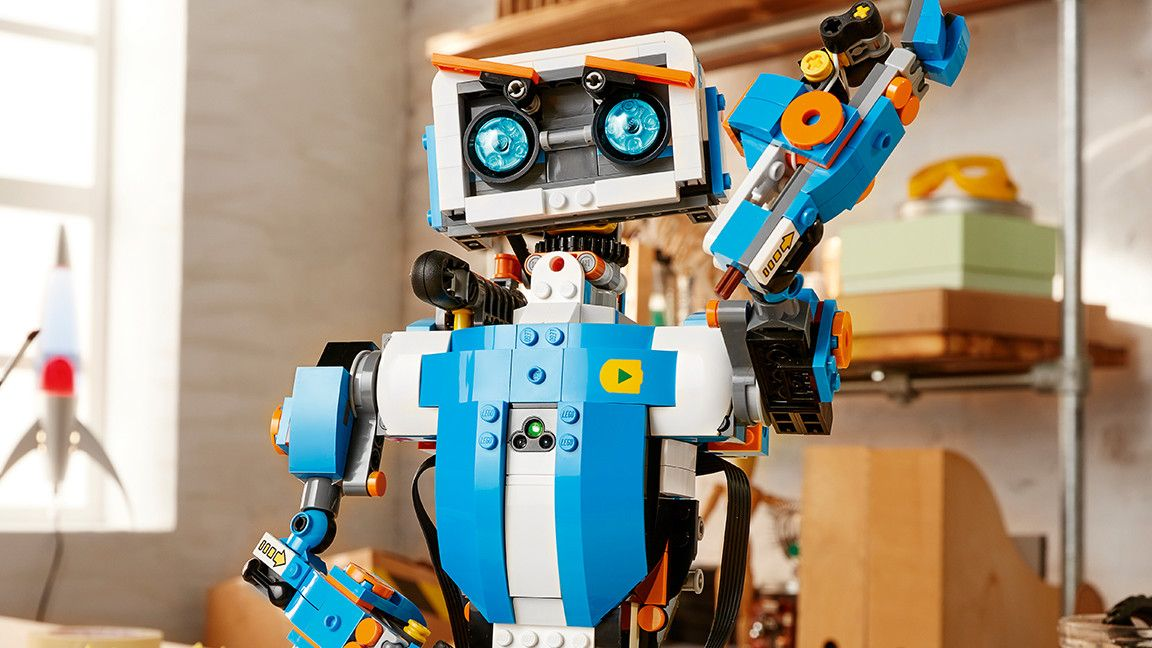
\includegraphics[width=0.8\textwidth]{07_vernie.jpg}};
            \node (led) [
                circle,
                draw = textColor,
                ultra thick,
                minimum size = 0.8cm,
                yshift = -1.15cm,
                xshift = -0.5cm,
            ] {};

            \node (text) [
                rectangle,
                xshift = -3cm,
                yshift = 1.5cm,
            ] {\textbf{LED}};

            \draw[arrow, ultra thick] (text) to[bend right] (led);

        \end{tikzpicture}

        \caption{Position of \ac{LED} on the Vernie robot.}
        \label{fig:vernie}
    \end{figure}
    
